\newcommand{\TeamNo}{31}

\newcommand{\HWno}{02}

\newcommand{\AuthorOneName}{Merve Nur Öztürk}
\newcommand{\AuthorOneID}{2311322}

\newcommand{\AuthorTwoName}{Atakan Süslü}
\newcommand{\AuthorTwoID}{2311371}

\newcommand{\AuthorThreeName}{Betül Rana Kuran}
\newcommand{\AuthorThreeID}{2311173}


\documentclass[letterpaper,12pt]{article}
\usepackage{tabularx} % extra features for tabular environment
\usepackage{amsmath}  % improve math presentation
\usepackage{amssymb}
\usepackage{xcolor}
\usepackage{float}
\usepackage[export]{adjustbox}
\usepackage{graphicx} % takes care of graphic including machinery
\usepackage[margin=1in,letterpaper]{geometry} % decreases margins
\usepackage{cite} % takes care of citations

\begin{document}
\begin{center}
AE 305, 2020-21 Fall \hfill \textbf{HW \HWno} \hfill \textbf{Team \TeamNo} \\
\noindent\rule{\textwidth}{0.4pt}
\begin{tabular}{p{0.33\textwidth} | p{0.33\textwidth} | p{0.33\textwidth} }
	\AuthorOneName&\AuthorTwoName&\AuthorThreeName\\
	\textit{\AuthorOneID}&\textit{\AuthorTwoID}&\textit{\AuthorThreeID}
\end{tabular}
\noindent\rule{\textwidth}{0.4pt}
\end{center}

%Report start

\section{Introduction}

Numerical methods, such as Runge Kutta Method, are widely used to solve differential equations when an
analytical solution is not possible or time-consuming. $4^{th}$ order Runge-Kutta Method is one of the
numerical methods which gives quite accurate results due to its small truncation error. In this homework,
a solid propellent rocket is given, and its chamber pressure $p_c$, burn rate $\dot{r}$, and the specific
impulse $I_{sp}$ are asked to be calculated with this method until the chamber pressure $p_c$ becomes equal 
to the atmospheric pressure $p_a$, with different time step sizes and different nozzle throat radiuses.

This equation gives the rate of the chamber pressure of the given rocket with a constant burn temperature
$T_c$:

\begin{equation}
	\frac{dp_c}{dt} = \frac{RT_c}{V_c}(\dot{m_{bs}} - \dot{m_{ce}} - \rho_{c}\dot{V_c})
\end{equation}

It is assumed that the propellant inner surface is circular and between the chamber exit and nozzle throat
no gas mass accumulates ($\dot{m_{ce}} = \dot{m_n}$). Moreover, writing $\dot{m_{bs}} = \rho_{p}2\pi rL\dot{r}$,
and $V_c = \pi r^{2}L$, the equation becomes:

\begin{equation}
	\frac{dp_c}{dt} = RT_c[\frac{2\dot{r}}{r}(\rho_{p} - \rho_{c}) - \frac{\dot{m_n}}{\pi r^{2}L}]
\end{equation}

It is given that $\dot{r} = ap_c^{n}$, and $\dot{m_n} = p_cA^{*}\sqrt{\frac{\gamma}{RT_c}}(\frac{\gamma +1}{2})^{-\frac{\gamma +1}{2(\gamma -1)}}$
where $A^{*}$ is the nozzle throat area. Furthermore, though at first it was assumed that the propellant 
inner surface is circular, it is more of a complex shape. Thus, a propellant design dependent factor
$f_{cor}(r)$ is used to simply approach to original characteristics. Then, the equations for the rate
of chamber pressure, and the rate of equivalent radius r become:

\begin{equation}
	\boxed{\frac{dp_c}{dt} = RT_c[f_{cor}(r)\frac{2ap_c^{n}}{r}(\rho_{p} - \frac{p_c}{RT_c}) - \frac{p_cA^{*}}{\pi r^{2}L}\sqrt{\frac{\gamma}{RT_c}}(\frac{\gamma +1}{2})^{-\frac{\gamma +1}{2(\gamma -1)}}]}
\end{equation}

\begin{equation}
	\boxed{\frac{dr}{dt} = ap_c^{n}}
\end{equation}

Specific impulse is also asked to be calculated, and its formula is:

\begin{equation}
	\boxed{I_{sp} = \frac{1}{g}\sqrt{\frac{2\gamma RT_c}{\gamma -1}[1-(\frac{p_a}{p_c})^{\frac{\gamma -1}{\gamma}}]}}
\end{equation}

\section{Method}
\subsection{Classical Fourth-order RK Method}
Basic form of RK method is :
\begin{equation}
	y_{i+1} = y_i + \Phi(x_i, y_i, \Delta x) \Delta x
	\label{eqn:rk}  
\end{equation} 
$\Phi$ can be defined as weighted slope function or increment function. It can be expressed as:
\begin{equation}
	\Phi = a_1k_1 + a_2k_2 + ... + a_nk_n
\end{equation}
where $k_1, k_2, ..., k_n$ are slopes, $a_1, a_2, ..., a_n$  are weights.\\
In classical fourth-order RK method, four slopes is calculated for each interval. Also, weights are equal to $1/6, 1/3, 1/3, 1/6$
, respectively. In the homework, there is the system of ordinary differential equations, $\frac{dy_i}{dt}$ and $\frac{dr_i}{dt}$. 
Therefore, RK method becomes:
\begin{eqnarray}
	y_{1,i+1}&=&y_{1,i} + \frac{1}{6}(k_{1,1} + 2k_{2,1} + 2k_{3,1} + k_{4,1})\Delta x \nonumber \\
	y_{2,i+1}&=&y_{2,i} + \frac{1}{6}(k_{1,2} + 2k_{2,2} + 2k_{3,2} + k_{4,2})\Delta x \nonumber \\
	\mbox{Stage 1: }k_{1,1}&=&f_1(x_i, y_{1,i}, y_{2,i} ) \nonumber \\
	k_{1,2}&=&f_2(x_i, y_{1,i}, y_{2,i}) \nonumber \\
	y^{*}_1 &=& y_{1,i} + k_{1,1}(p_1\Delta x) \nonumber \\
	y^{*}_2 &=& y_{2,i} + k_{1,2}(p_1\Delta x) \nonumber \\
	\mbox{Stage 2: }k_{2,1}&=&f_1(x_{i+(p_1\Delta x)} ,y^{*}_1, y^{*}_2 ) \nonumber \\
	k_{2,2}&=&f_2(x_{i+(p_1\Delta x)} ,y^{*}_1, y^{*}_2 ) \nonumber \\
	y^{**}_1&=&y_{1,i} + k_{2,1}(p_2\Delta x) \nonumber \\
	y^{**}_2&=&y_{2,i} + k_{2,2}(p_2\Delta x) \nonumber \\
	\mbox{Stage 3: }k_{3,1}&=&f_1(x_{i+(p_2\Delta x)} ,y^{**}_1, y^{**}_2 ) \nonumber \\
	k_{3,2}&=&f_2(x_{i+(p_2\Delta x)} ,y^{**}_1, y^{**}_2 ) \nonumber \\
	y^{***}_1&=&y_{1,i} + k_{1,3}(p_3\Delta x) \nonumber \\
	y^{***}_2&=&y_{2,i} + k_{2,3}(p_3\Delta x) \nonumber \\
	\mbox{Stage 4: }k_{4,1}&=&f_1(x_{i+(p_1\Delta x)} ,y^{**}_1, y^{**}_2 ) \nonumber \\
	k_{4,2}&=&f_2(x_{i+(p_3\Delta x)} ,y^{***}_1, y^{***}_2 ) \nonumber
\end{eqnarray}
where $y\prime = f(x_i,y_i)$ and $p_1=p_2=1/2$, $p_3=1$.\\
At every stage, first the slope of $r_i$ ($k_{n,1}$) and  $p_{c_{i}}$ ($k_{n,2}$) at $p_n$ fraction of interval is calculated. 
Then, temporary $p_{c_{i+(p_n\Delta x)}}$ and $r_{i+(p_n\Delta x)}$ values are determined, which enables to calculate the next 
slopes $p_{n+1}$ fraction of the same interval. After four stages, weighted slopes are determined. By substituting known 
variables into Equation \ref{eqn:rk}, next value $r_{i+1}$ and $p_{c_{i+1}}$ are calculated. 
\subsection{Adaptive RK Method}
\label{section:adaptive}
Sometimes the change in solutions may not be consistent. Small step sizes cause the increase in the number of steps, which leads to
rise in round off errors, whereas large step sizes cause the larger truncation errors. Adaptive RK method is used to capture important
changes in the solution, at the same time it prevents overkill with small step sizes. It basically provides appropriate step sizes 
according to the change in solution. In adaptive step size control, first the local truncation error, $E_o$, is calculated. In this 
homework, $E_o$ is determined by using the difference between RK2 method and RK4 method.
\begin{equation}
	E_o = \frac{y_{RK4}-y_{RK2}}{y_{RK4}}
\end{equation}
Then, to check whether step size is appropriate or not, some comparisons are made:
\begin{eqnarray}
	1 < \left\lvert \frac{E_{allowed}}{E_o} \right\rvert &<& 5 \textrm{, leave $\Delta x$ uncahnged} \nonumber \\
	\left\lvert \frac{E_{allowed}}{E_o} \right\rvert &>& 5  \textrm{, increase $\Delta x$ by a factor of 2} \nonumber \\
	\left\lvert \frac{E_{allowed}}{E_o} \right\rvert &<& 1  \textrm{, decrease $\Delta x$ by a factor of 2 and redo the current step} \nonumber 
\end{eqnarray}
where $E_{allowed}$ is the allowed percent error tolerance and equal to $10^{-4}$  .


\newpage

\section{Results and Discussion}
\subsection{Calculation of $p_c$, $\dot{r}$ and $I_{sp}$ with different time step sizes}

\begin{figure} [ht]
	\centering
	\includegraphics[height = 8.4cm]{graphs/q1_pc.eps}
	\caption{Calculated $p_c$ values using $4^{th}$ order RK method with three different step sizes.}
     \label{fig:q1pc}
\end{figure}

This figure demonstrates how the chamber pressure $p_c$ changes as time progresses. As it can be seen in 
Figure \ref{fig:q1pc}, there are three curves, one for each step size. However,
there is no significant difference between the curves, which results from the high degree of accuracy
provided by the $4^{th}$ order RK method. This is because the truncation error for this method is so
small that its effect on the results can be nearly neglected. In addition, using smaller step sizes
helps to calculate more precisely, and it is obvious that the step sizes used for this problem are small
enough. As a result, the values obtained for the chamber pressure $p_c$ of the rocket were approximately
the same for three different step sizes.

\newpage

\begin{figure} [!h]
	\centering
	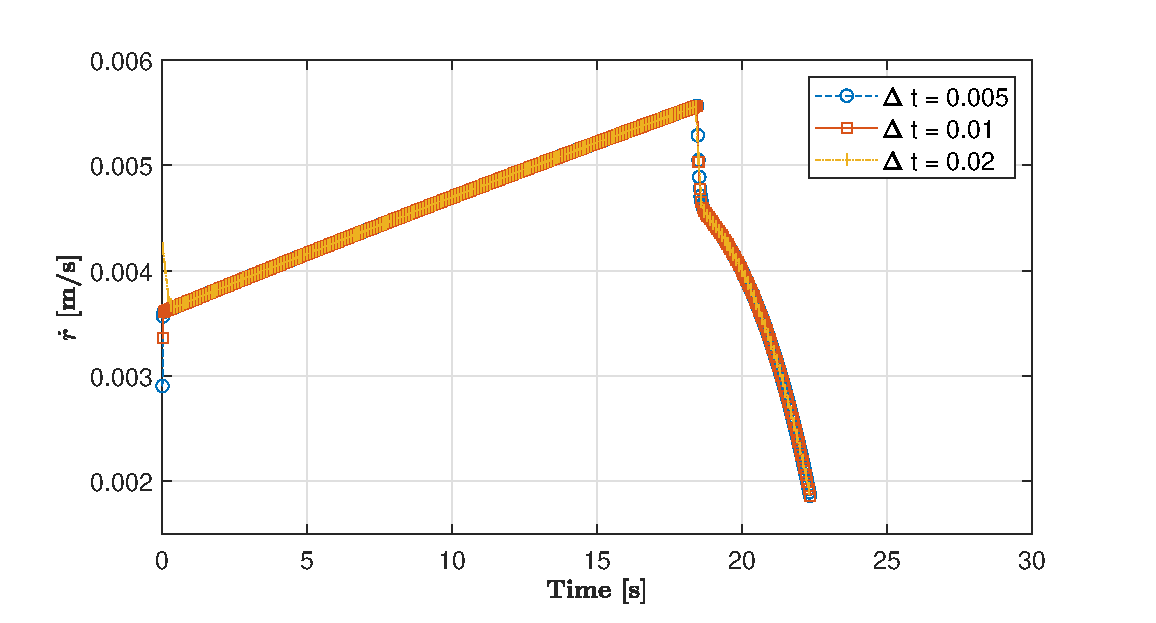
\includegraphics[height = 8.4cm]{graphs/q1_rdot.eps}
	\caption{Calculated $\dot{r}$ values using $4^{th}$ order RK method with three different step sizes.}
	\label{fig:q1rdot}
\end{figure}

\begin{figure} [!h]
	\centering
	\includegraphics[height = 8.4cm]{graphs/q1_isp.eps}
	\caption{Calculated $I_{sp}$ values using $4^{th}$ order RK method with three different step sizes.}
	\label{fig:q1Isp}
\end{figure}

As it was for $p_c$, there are three curves, one for each step size, for also the rate of equvalent radius
$\dot{r}$ and the specific impulse $I_{sp}$ in Figure \ref{fig:q1rdot} and in Figure \ref{fig:q1Isp}, respectively. 
Since the conditions are the same as mentioned above, the values calculated for $\dot{r}$ and $I_{sp}$ does not 
experience a major change for different step sizes. The point is, the accuracy of the results obtained by using RK4 Method
is remarkably of a high degree no matter what size of a time step is used.

\subsection{Q2}
\begin{figure}[!h]
	\centering
	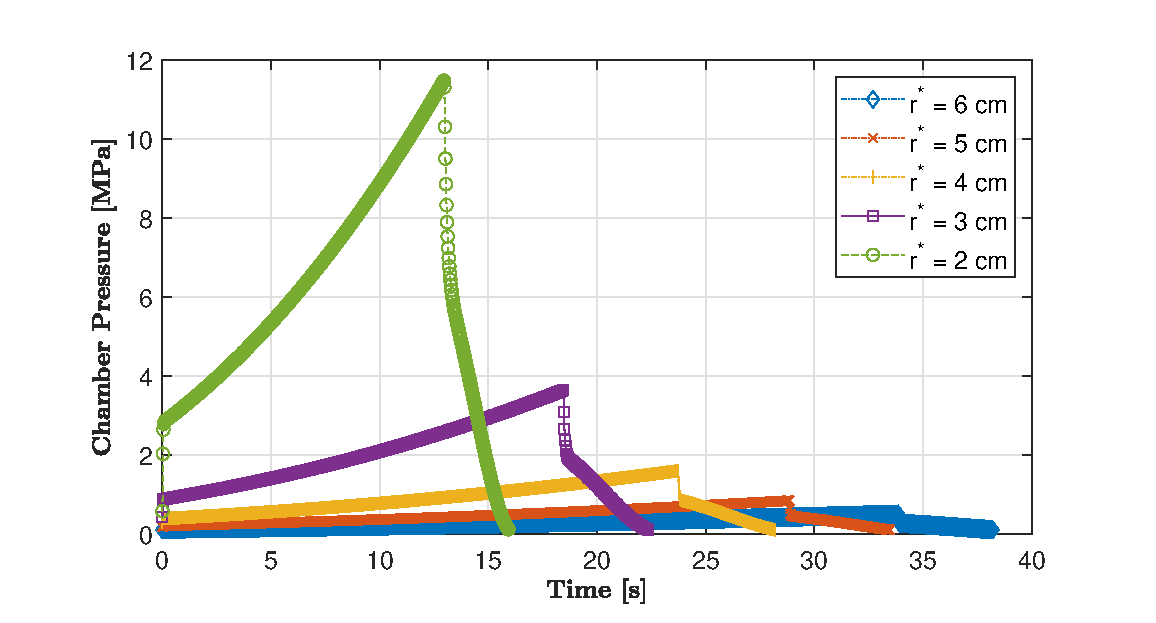
\includegraphics[height = 8.5cm]{graphs/q2_pc.eps}
	\label{fig:q2p_cp}
\end{figure}
As can be cleary concluded from the graph, decreasing the radius of the nozzle leads to increase in both maximum chamber pressure
and needed time for chamber pressure to reach the ambient pressure. The reason of that is reducing the radius causes exponential
decrease in the area of nozzle. As the area of nozzle becomes higher means the lower chamber pressure. Therefore, maximum chamber
pressures incline, exponentially with reducing radius of the throat. Also, since nozzle area is grow, the time to total mass flow 
of the gas exits from the nozzle extends. Because with higher radiuses, the mass flow rate reduces.
\newpage
\begin{figure}[!h]
	\centering
	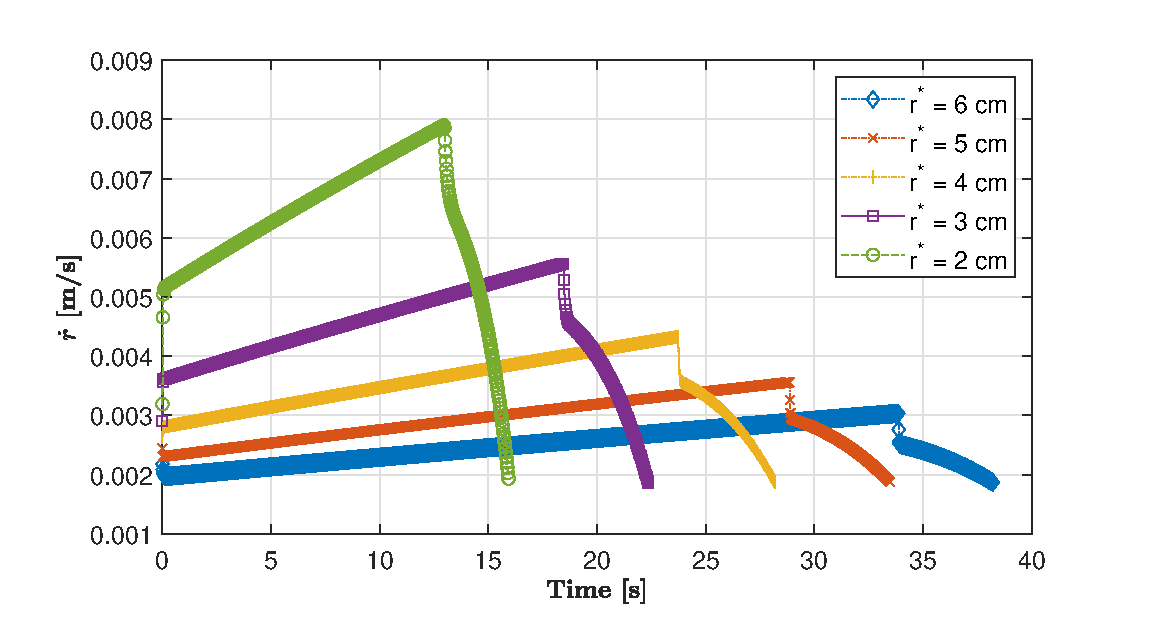
\includegraphics[height = 8.5cm]{graphs/q2_rdot.eps}
	\label{fig:q2r_dot}
\end{figure}
$\dot r$ gives the similar reaction to the different nozzle throat radiuses with the chamber of pressure. Lower radiuses cause higher 
maximum burn rates and longer times to reach the ambient pressure. On the other hand, unlike to curves in Figure \ref{fig:q2p_cp}, every 
curve in the Figure \ref{fig:q2r_dot} are approximately linear with different slopes, which are grow with reducing radiuses. The reason 
of both conclusions can be explained with the same equation. $\dot{r}$ is proportional to $p_c$; therefore, both of them gives 
the similar response to difference throat radiuses. However, since the propallent burn rate exponent in the equationis smaller than 1, 
the growth in the maximum burn rates in Figure \ref{fig:q2p_cp} is less dramatic than the maximum chamber pressures in Figure 
\ref{fig:q2r_dot}. The result of that is nearly linear curves.

\begin{figure}[!h]
	\centering
	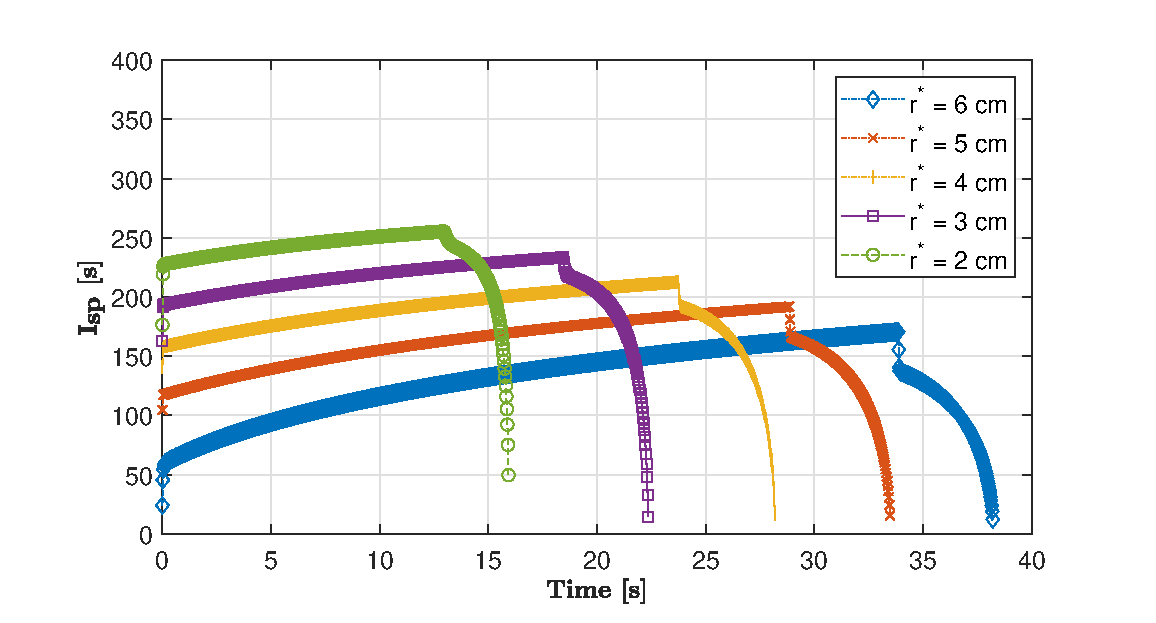
\includegraphics[height = 8.5cm]{graphs/q2_isp.eps}
	\label{fig:q2I_sp}
\end{figure}
In Figure \ref{fig:q2I_sp}, it is shown that maximum specific impulse reduces and time to reach the ambient pressure becomes longer with
growing throat radiuses. This answers is similar to the answer of $p_c$ It can be explained by Equation. As $p_c$ increases, the value in
the square root is increases. Therefore, the specific impulse increases. However, since the exponent of $p_c$ is less than 1 the growth of 
curves are different from curves of $p_c$ in Figure \ref{fig:q2p_cp}

\subsection{Calculation using adaptive stepping}

\begin{figure}[!h]
	\centering
	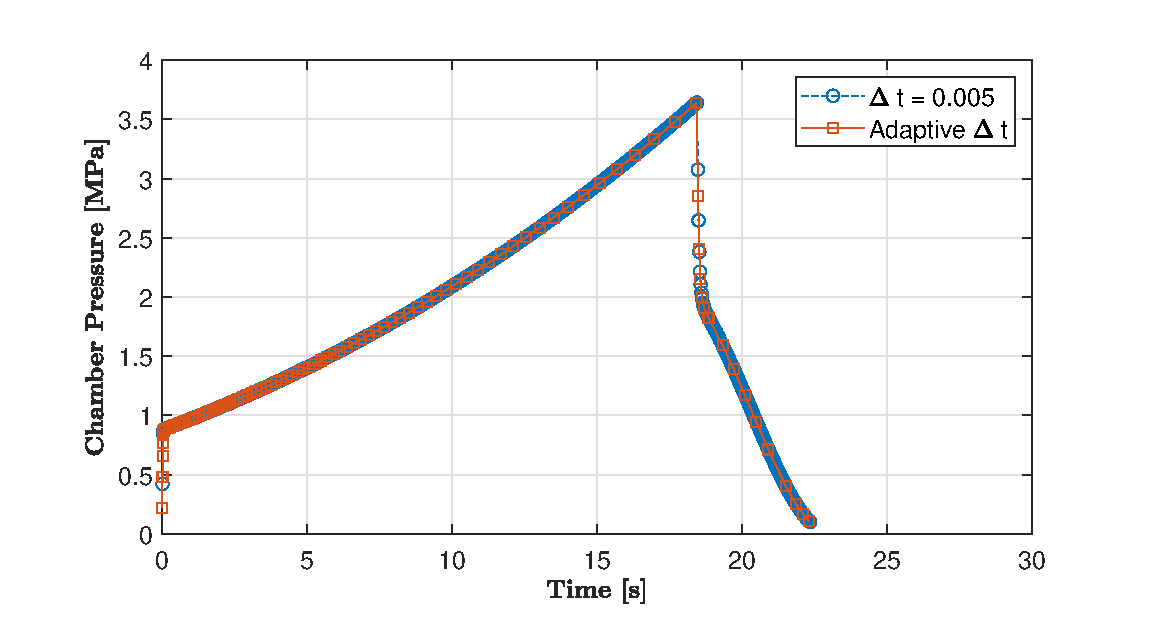
\includegraphics[height = 8.5 cm]{graphs/bonus_pc.eps}
	\caption{Chamber pressure versus time graph with constant and adaptive step size.}
	\label{fig:bonus_cp}
\end{figure}

It can be seen from Figures \ref{fig:bonus_cp}, \ref{fig:bonus_isp} and \ref{fig:bonus_rdot} that when adaptive stepping is 
applied with allowed percent tolerance $E_o = 0.0001$, linear parts can be calculated with less steps without losing any accuracy as discussed in 
Section \ref{section:adaptive}. When there is a sudden change, step size gets smaller accordingly and results can be calculated correctly in that region.

It can be seen from Table \ref{tbl:timeint} that using adaptive stepping reduces total number of time intervals needed significantly.
Although results are calculated three times for each time interval(twice for determining the step size and once for calculating result) 
using adaptive stepping approach, number of time intervals needed are much lower than constant step size approach. Therefore adaptive stepping is 
computationally cheaper without losing accuracy. 


\begin{table}[!h]
	\begin{center}
	\caption{Total number of time intervals needed for computations.}
	\vspace{1em}
	\label{tbl:timeint}
	\begin{tabular}{|c|c|} 
	\hline
	\multicolumn{1}{|c|}{\bf{Stepping Approach}} & \multicolumn{1}{c|}{\bf{Number of time intervals needed}} \\
	\hline
	Constant $\Delta t = 0.005$ &   4470 \\ \hline
	Adaptive Stepping with initial $\Delta t = 0.005$ &   462 \\ \hline
	\end{tabular}
	\end{center}
\end{table}


\newpage

\begin{figure}[!h]
	\centering
	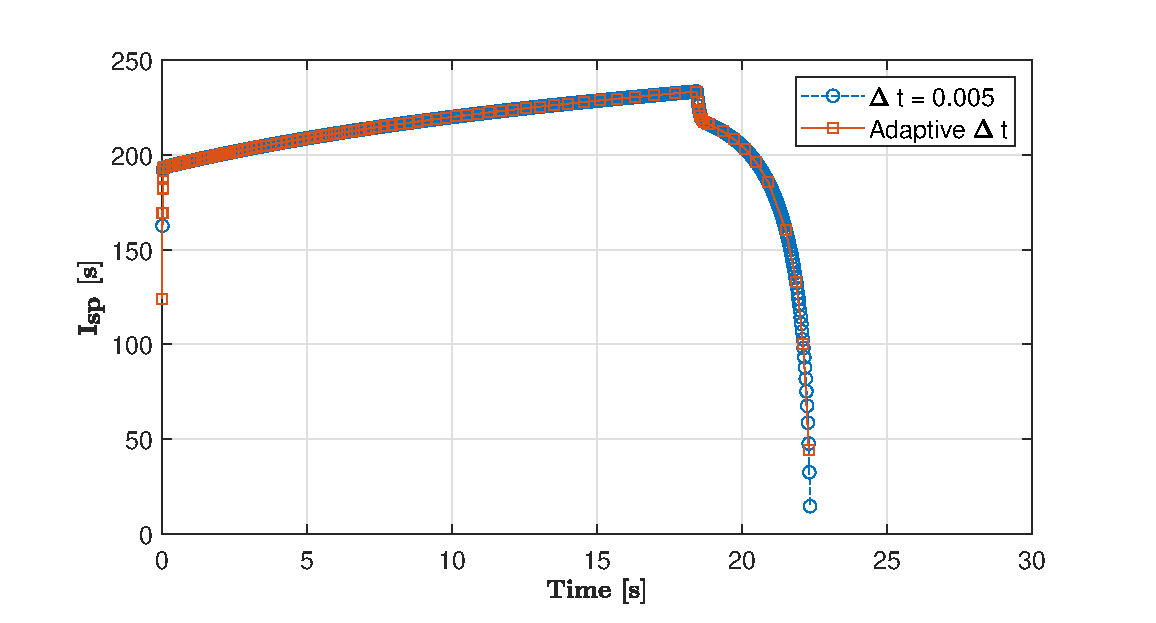
\includegraphics[height = 8.5 cm]{graphs/bonus_isp.eps}
	\caption{Specific impulse versus time graph with constant and adaptive step size.}
	\label{fig:bonus_isp}
\end{figure}

\begin{figure}[!h]
	\centering
	\includegraphics[height = 8.5 cm]{graphs/bonus_rdot.eps}
	\caption{Burn rate versus time graph with constant and adaptive step size.}
	\label{fig:bonus_rdot}
\end{figure}

%\section{Conclusion}

\end{document}